\documentclass[10pt,a4paper]{article}
\usepackage[T1]{fontenc}
\usepackage[a4paper]{geometry}
\usepackage{xcolor}
\usepackage{amssymb}
\usepackage{amsmath}
\usepackage{graphicx}
\usepackage{tabularx}
\usepackage{multirow}
\usepackage{subfigure}
\usepackage{verbatim}
\usepackage{fancyhdr}
\usepackage{listings}
\usepackage{../common/espacs}

%\input{../common/commands.tex}

\newcommand*{\vect}[1]{\boldsymbol{#1}}
\newcommand*{\mat}[1]{\boldsymbol{#1}}

\title{Exercise Session 5}
\date{November 9, 2012}

\pagestyle{fancy}
\headheight 35pt

\begin{document}
\lstset{language=[ISO]C++}
\maketitle

\section*{Data mining: $k$-means clustering}

$k$-means clustering is a common method used in data mining, which aims to
partition $N$ objects into $k$ clusters, with $k << N$. The clusters are built
such as each object belongs to the \emph{nearest} cluster, so there must be a
notion of distance between objects.

An object example can be a point in $\RR^n$ equipped with the Euclidean norm. In
this case the distance would be computed with respect to the centroid of the
cluster and the space would be partitioned in Voronoi cells. The approach is
however more genaral, it can be applied to any set of objcts with a kwnoledge of
a distance between then, e.g. functions in a suitable space and a suitable norm,
etc.

%%%%%%%%%%%%%%
\begin{figure}[htb]
\centering
$\vcenter{\hbox{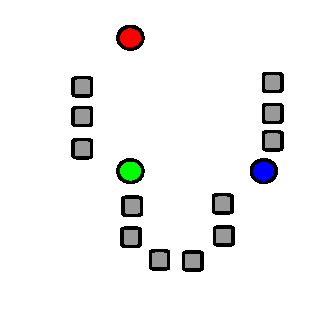
\includegraphics[width=.3\textwidth]{fig/wiki1}}}$
\hfil
$\vcenter{\hbox{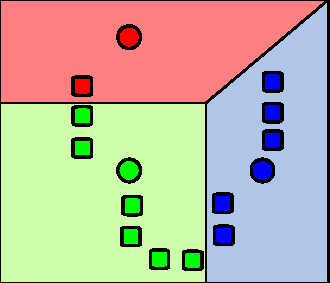
\includegraphics[width=.3\textwidth]{fig/wiki2}}}$
\\[1ex]
$\vcenter{\hbox{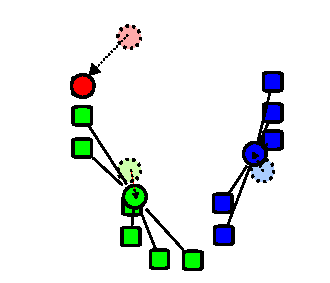
\includegraphics[width=.3\textwidth]{fig/wiki3}}}$
\hfil
$\vcenter{\hbox{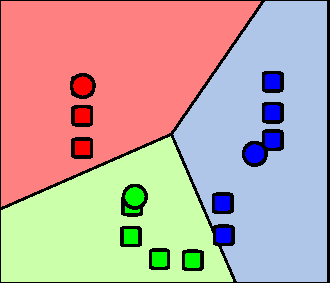
\includegraphics[width=.3\textwidth]{fig/wiki4}}}$
\caption{$k$-means algorithm in $\RR^2$. The squares represent the objects to be
clustered, while the circles represent the centroids of the partitions. Each
}
\label{fig:alg}
\end{figure}
%%%%%%%%%%%%%%
The problem is NP-hard, but an algorithm can be devised in order to approach a
local optimum. The algorithm is depicted in Fig. \ref{fig:alg} for the case of
points in $\RR^2$. Given a set of initial centroids, the objects are associated
to the nearest centroid to build up the clusters. Afterwords, the centroid is
updated to the point that minimizes the distance between the objects that belong
to the partition. In the case of the Euclidean norm it will be the barycenter of
the points in the cluster. This concludes a step of the algorithm, that is
repeated starting again assigning the points to the nearest centroid.

The algorithm stops when the clusters are fixed: when all the points are again
assigned to the same partition, the update of the centroids gives a null
increment. Note that, since we only reach a local optimum, the solution is
dependent on the choice of the initial guess for the centroids.

\section*{Exercise 1}

Implement a random walk in one dimension, using the following tips:
\begin{itemize}
  \item use a \cpp{map} to store the distribution of particles.
  \item use as starting configuration a Dirac delta --- approximated with
  $10000$ particles located at zero (use a much smaller value until the code
  is functioning properly).
  \item consider that the particles move by 1 or -1 at each time step,
  \item use a \cpp{discrete_distribution} to emulate the random motion, with
  equal probability of moving forwards or backwards.
  \item simulate 20 time steps.
  \ item print out the distribution to screen and to file, in order to plot it
  in \texttt{gnuplot}.
  \item plot also the fundamental solution in gnuplot to compare the result,
  remembering that $D = \frac{h^2}{2t}$.
  \item check what happens if the distrubution is biased towards one direction,
  or if the particle is allowed to remain in the same position, without	moving.
\end{itemize}

\section*{Exercise 2}

Implement a class that performs MonteCarlo (MC) integration, using a suitable
probability distribution.



\section*{Solution}

\begin{enumerate}

\item Main aspects of the solution for question 1:

\begin{itemize}

\item Both declarations and definitions of templated classes and methods mus be in a header files, for this reason we collected all the class declarations and implementations in one single header file. Other code organizations are possible as explained in the lectures.

\item In a class template derived names are 
resolved only when a template class is instantiated 
so methods and attributes in the derived classes {\tt Bisection}, {\tt Newton}, and {\tt Robust} that are inherited from the base class {\tt IterativeMethod}
must be prepended by {\tt this->} so that the compiler
can understand they are dependent identifiers and only try to resolve them when the templated classes are instantiated.

\item For a similar reason the typedefs in the base
class need to be fully qualified when used in the derived classes.

\item Using the {\tt STL} class template {\tt numeric\_limits}.

\end{itemize}

Main file:

\lstinputlisting{ex8_sol1/bn.cpp}

Header defining all the class templates:
\lstinputlisting{ex8_sol1/iterativeMethod.hpp}

\item Main aspects of the solution for question 2:

\begin{itemize}
\item Notice that, unless specifying {\tt -std=c++11}, a space is required when two {\tt >} 
symbols appear consecutively in a template parameter list.
\end{itemize}

Main file:

\lstinputlisting{ex8_sol2/bn.cpp}

Header defining all the class templates:
\lstinputlisting{ex8_sol2/iterativeMethod.hpp}

\end{enumerate}






\end{document}
